% =====================================================================
%  Emergent Causal Order from Entanglement: A Pedagogical Introduction
%
%  Self-contained pedagogical exposition of the hypothesis and
%  methodology behind the Phase 5 numerical experiment in
%  caset.quantum.  Builds from undergraduate linear algebra and quantum
%  mechanics up through the lattice Schwinger model and tensor-network
%  time evolution, with the goal that a motivated reader can follow the
%  argument end-to-end without consulting outside sources.
%
%  Build:    pdflatex emergent_causal_order.tex   (run twice for refs)
% =====================================================================

\documentclass[11pt,a4paper]{article}

\usepackage[utf8]{inputenc}
\usepackage[T1]{fontenc}
\usepackage{lmodern}
\usepackage{microtype}
\usepackage[a4paper,margin=1in]{geometry}

\usepackage{amsmath,amssymb,amsthm,mathtools}
\usepackage{bm}
\usepackage{enumitem}
\usepackage{booktabs}
\usepackage{array}
\usepackage{tikz}
\usetikzlibrary{arrows.meta,positioning,calc,decorations.pathreplacing}
\usepackage{hyperref}
\hypersetup{
  colorlinks=true,
  linkcolor=blue!50!black,
  urlcolor=blue!50!black,
  citecolor=blue!50!black,
}

% --- Theorem-like environments ---------------------------------------
\theoremstyle{definition}
\newtheorem{definition}{Definition}[section]
\newtheorem{example}[definition]{Example}

\theoremstyle{plain}
\newtheorem{theorem}[definition]{Theorem}
\newtheorem{proposition}[definition]{Proposition}
\newtheorem{lemma}[definition]{Lemma}

\theoremstyle{remark}
\newtheorem*{remark}{Remark}

% --- Macros ----------------------------------------------------------
\newcommand{\ket}[1]{\lvert #1 \rangle}
\newcommand{\bra}[1]{\langle #1 \rvert}
\newcommand{\braket}[2]{\langle #1 \mid #2 \rangle}
\newcommand{\norm}[1]{\lVert #1 \rVert}
\newcommand{\abs}[1]{\lvert #1 \rvert}
\newcommand{\Tr}{\operatorname{Tr}}
\newcommand{\diag}{\operatorname{diag}}
\newcommand{\Hilb}{\mathcal{H}}
\newcommand{\real}{\mathbb{R}}
\newcommand{\complex}{\mathbb{C}}
\newcommand{\nat}{\mathbb{N}}
\newcommand{\maj}{\mathrm{maj}}
\newcommand{\LR}{\mathrm{LR}}
\newcommand{\cs}{\mathrm{cs}}
\newcommand{\preceqmaj}{\preceq_{\maj}}
\newcommand{\preceqLR}{\preceq_{\LR}}
\newcommand{\preceqcs}{\preceq_{\cs}}
\DeclareMathOperator{\spec}{spec}
\DeclareMathOperator*{\argmin}{arg\,min}

\title{Emergent Causal Order from Entanglement\\
\large A Pedagogical Introduction to a Tensor-Network Hypothesis Test}

\author{}
\date{}

\begin{document}
\maketitle

\begin{abstract}
A common slogan in modern theoretical physics is that ``spacetime is built
from entanglement''.  Stripped of mystique, the claim is that the causal
and geometric structure we see in the macroscopic world might be a
derived feature of how a quantum state is correlated across its parts.
This paper presents, from first principles, one concrete way of taking
that slogan seriously enough to test on a small computer.  We work in
$1{+}1$ dimensional lattice quantum electrodynamics, where a
tensor-network simulation can produce the full quantum state of an
evolving particle--antiparticle pair on a $20$-site chain.  From that
state we read off three different partial orders on space-time events:
the order induced by the lattice's own causal structure, the order
induced by the Lieb--Robinson bound, and an order built from the
entanglement structure via Nielsen majorization.  The hypothesis we
test is whether the three orders coincide.  The paper builds every
ingredient from undergraduate linear algebra and quantum mechanics; no
outside references are required to follow the argument or interpret
the result.
\end{abstract}

\tableofcontents

% =====================================================================
\section{Introduction}\label{sec:intro}

The question we want to answer is a small, sharply-posed, numerical
version of a much grander question.  Let us start with the grand
version and then reduce it.

\paragraph{The grand question.}
General relativity says spacetime has a causal structure: every point
has a past, a future, and a set of points spacelike-separated from it.
Quantum mechanics says quantum states can be entangled: knowing part of
a state restricts what the other part can be.  Various lines of
research over the past two decades have suggested that these are not
two independent facts, but that the causal structure of spacetime
might be \emph{built out of} the entanglement structure of an
underlying quantum state.  The most ambitious version of the claim is
that there is no spacetime at the bottom layer of physics; there are
only quantum correlations, and what we call ``causality'' is a
coarse-grained reading of those correlations.

\paragraph{Why we cannot directly test it.}
There is no version of quantum gravity we trust well enough to
simulate.  Even if there were, the gulf between Planck-scale physics
and the experimental scales we can probe is enormous.  Any direct test
of the grand claim is, for the foreseeable future, out of reach.

\paragraph{The small question.}
We can, however, ask a much more limited question that is in principle
testable today.  Take any quantum many-body system on a discrete
lattice.  Such a system has its own intrinsic causal structure, given
by the lattice on which the Hamiltonian acts.  It also has, via the
Lieb--Robinson theorem, a strict speed limit on how fast information
can propagate.  A real-time-evolved state of such a system is
entangled, and the entanglement, when measured between any two
contiguous regions, has a quantitative structure: the Schmidt
spectrum.  We will define an ordering relation among space-time
``cuts'' based purely on those Schmidt spectra.  And we will ask the
following:
\begin{quote}\itshape
  Is the partial order one reads off from the entanglement structure
  the same as the partial order one reads off from causality?
\end{quote}
This question is finite, well-posed, and amenable to a tensor-network
simulation that runs in under a minute on a laptop.  This paper is
about how to set up that test, what the right answer would tell us,
and what the actual answer turns out to be.

\paragraph{Roadmap.}
Sections~\ref{sec:math}--\ref{sec:majorization} build the mathematical
machinery: probability vectors, partial orders, density matrices, the
Schmidt decomposition, and majorization.
Section~\ref{sec:schwinger} introduces the lattice Schwinger model,
the smallest non-trivial gauge theory, as the physical test bed.
Section~\ref{sec:causal-lattice} explains the Lieb--Robinson bound and
causal sets.  Section~\ref{sec:three-orders} brings the three partial
orders together and states the hypothesis precisely.
Sections~\ref{sec:tn}--\ref{sec:metrics} describe the numerical
machinery and comparison statistics.  Section~\ref{sec:results}
presents the actual result of the experiment.
Sections~\ref{sec:discussion}--\ref{sec:outlook} interpret it and lay
out what would distinguish the two natural readings.  An appendix
collects notation.

\paragraph{Prerequisites.}
Linear algebra over the complex numbers; the bra--ket formalism of
quantum mechanics at the level of a first undergraduate course; a
willingness to take a few canonical results (Lieb--Robinson,
Nielsen's majorization theorem, the existence of efficient
matrix-product-state algorithms) on faith.  Where a result is stated
without proof we will say so explicitly and explain enough about its
content that the rest of the paper does not depend on the proof.

% =====================================================================
\section{Mathematical preliminaries}\label{sec:math}

\subsection{Probability vectors}

A \emph{probability vector} of length $d$ is a tuple
$p = (p_1, \ldots, p_d)$ with $p_i \ge 0$ and $\sum_i p_i = 1$.  Two
probability vectors of different lengths can be compared by
zero-padding the shorter to the length of the longer; we adopt this
convention throughout.  The set of probability vectors on $d$ symbols
is the standard $(d{-}1)$-simplex $\Delta_{d-1}$.

Two extremes are useful to keep in mind:
\begin{itemize}[nosep]
  \item the \emph{point distribution} $(1, 0, \ldots, 0)$, corresponding
        to a deterministic outcome;
  \item the \emph{uniform distribution} $(\tfrac1d, \ldots, \tfrac1d)$,
        corresponding to maximal uncertainty among $d$ outcomes.
\end{itemize}
We will see that pure quantum states attached to bipartitions produce
probability vectors via their Schmidt spectrum.

\subsection{Partial orders}

A \emph{partial order} on a set $S$ is a relation $\preceq$ such that for
all $a, b, c \in S$:
\begin{enumerate}[label=(\roman*),nosep]
  \item $a \preceq a$ (reflexivity);
  \item $a \preceq b$ and $b \preceq a$ imply $a = b$ (antisymmetry);
  \item $a \preceq b$ and $b \preceq c$ imply $a \preceq c$
        (transitivity).
\end{enumerate}
We say $a$ and $b$ are \emph{comparable} if $a \preceq b$ or
$b \preceq a$, and \emph{incomparable} otherwise.  The familiar
$\le$ on real numbers is a \emph{total order} (every pair is
comparable); a partial order need not be total.

A partial order on a finite set is conveniently visualized by its
\emph{Hasse diagram}: a graph with one vertex per element and an edge
$a \to b$ whenever $a \preceq b$ and there is no $c \ne a,b$ with
$a \preceq c \preceq b$ (we say $a$ is \emph{covered by} $b$).
Transitive consequences are implied by following multiple edges.

\begin{example}[Subsets of a $3$-element set]
Take $S = \{\emptyset, \{1\}, \{2\}, \{1,2\}, \{1,3\}, \{1,2,3\}\}$
ordered by $\subseteq$.  The Hasse diagram is shown in
Figure~\ref{fig:hasse-subset}.  Note that $\{2\}$ and $\{1,3\}$ are
incomparable: neither contains the other.
\end{example}

\begin{figure}[h]
\centering
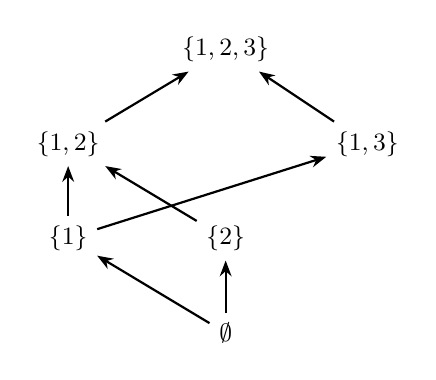
\begin{tikzpicture}[
  node distance=12mm and 14mm,
  every node/.style={font=\small},
  edge/.style={-{Stealth[length=2mm]}, thick},
]
  \node (e)   at (0, 0)   {$\emptyset$};
  \node (1)   at (-2, 1.2){$\{1\}$};
  \node (2)   at (0, 1.2) {$\{2\}$};
  \node (12)  at (-2, 2.4){$\{1,2\}$};
  \node (13)  at (1.8, 2.4){$\{1,3\}$};
  \node (123) at (0, 3.6) {$\{1,2,3\}$};
  \draw[edge] (e)  -- (1);
  \draw[edge] (e)  -- (2);
  \draw[edge] (1)  -- (12);
  \draw[edge] (2)  -- (12);
  \draw[edge] (1)  -- (13);
  \draw[edge] (12) -- (123);
  \draw[edge] (13) -- (123);
\end{tikzpicture}
\caption{Hasse diagram of a partial order on six subsets, ordered by
$\subseteq$.  Edges show the cover relation; transitive consequences
are implied.  $\{2\}$ and $\{1,3\}$ are incomparable.}
\label{fig:hasse-subset}
\end{figure}

\subsection{Comparing two partial orders}\label{ssec:kendall}

Given two partial orders $\preceq_a$ and $\preceq_b$ on the same finite
set $S$, we want a number that tells us how similar they are.  For each
unordered pair $\{x, y\} \subseteq S$ with $x \ne y$, exactly one of the
following holds in each order:
\begin{enumerate}[label=(\alph*),nosep]
  \item $x$ relates to $y$ (i.e.\ $x \preceq y$ or $y \preceq x$);
  \item $x$ and $y$ are incomparable.
\end{enumerate}
For pairs comparable in \emph{both} orders we can further ask whether
they relate the same way (\emph{concordant}) or in opposite ways
(\emph{discordant}).  Define
\begin{align}
  n_{cc} &= \#\{ \text{pairs comparable in both, agreeing in direction} \},\\
  n_{dd} &= \#\{ \text{pairs comparable in both, disagreeing in direction} \},\\
  n_a^o &= \#\{ \text{pairs comparable in $\preceq_a$ only} \},\\
  n_b^o &= \#\{ \text{pairs comparable in $\preceq_b$ only} \}.
\end{align}
The classical \emph{Kendall correlation coefficient} on the
both-comparable subset is
\begin{equation}\label{eq:kendall}
  \tau_{ab} = \frac{n_{cc} - n_{dd}}{n_{cc} + n_{dd}}
            \in [-1, 1].
\end{equation}
A value $\tau_{ab} = +1$ means the two orders agree wherever both
relate the pair; $\tau_{ab} = -1$ means they disagree everywhere; values
near $0$ mean the agreement and disagreement are roughly balanced.

The numbers $n_a^o$ and $n_b^o$ measure asymmetric disagreement:
``$\preceq_a$ relates this pair, $\preceq_b$ does not''.  We will
need both $\tau$ and the asymmetric counts in
Section~\ref{sec:metrics}; $\tau$ is informative when both orders
are dense, $n_a^o$ and $n_b^o$ are informative when one order is
much sparser than the other.

% =====================================================================
\section{Quantum states and the Schmidt decomposition}\label{sec:quantum}

\subsection{Pure states}

A quantum system has a complex Hilbert space $\Hilb$.  A pure state is
a unit vector $\ket{\psi} \in \Hilb$, defined up to an overall complex
phase.  Inner products are written $\braket{\phi}{\psi}$.  Operators
$O : \Hilb \to \Hilb$ have an adjoint $O^\dagger$; \emph{Hermitian}
operators ($O = O^\dagger$) play the role of observables; \emph{unitary}
operators ($U U^\dagger = I$) generate dynamics.

For finite-dimensional $\Hilb \cong \complex^d$ we will routinely fix
an orthonormal basis $\{\ket{i}\}_{i=1}^d$ and write
$\ket{\psi} = \sum_i c_i \ket{i}$ with $\sum_i \abs{c_i}^2 = 1$.

\subsection{Composite systems}

If two systems have Hilbert spaces $\Hilb_A$ and $\Hilb_B$, the
combined system has Hilbert space
$\Hilb_{AB} = \Hilb_A \otimes \Hilb_B$, the tensor product.
Concretely, if $\dim \Hilb_A = d_A$ and $\dim \Hilb_B = d_B$, then
$\dim \Hilb_{AB} = d_A \cdot d_B$, and a basis is
$\{\ket{i}_A \otimes \ket{j}_B\}_{i,j}$, abbreviated $\ket{i,j}$.

A general state of the joint system is
\begin{equation}\label{eq:joint}
  \ket{\Psi} = \sum_{i,j} \Psi_{ij} \, \ket{i,j},
  \qquad \sum_{i,j}\abs{\Psi_{ij}}^2 = 1.
\end{equation}
The matrix $\Psi$ of coefficients carries the entire correlation
structure between $A$ and $B$.

A state is called a \emph{product state} if it factorizes:
$\ket{\Psi} = \ket{\phi}_A \otimes \ket{\chi}_B$, equivalently
$\Psi_{ij} = \phi_i \chi_j$.  Otherwise it is \emph{entangled}.

\subsection{Reduced density matrices}

If we have access only to subsystem $A$ of the joint state $\ket{\Psi}$,
the relevant object is the \emph{reduced density matrix}
\begin{equation}\label{eq:rho}
  \rho_A = \Tr_B \ket{\Psi}\bra{\Psi},
\end{equation}
where $\Tr_B$ is the partial trace over $\Hilb_B$.  Concretely,
$(\rho_A)_{ii'} = \sum_j \Psi_{ij} \overline{\Psi_{i'j}}$, i.e.\
$\rho_A = \Psi \Psi^\dagger$ (treating $\Psi$ as a $d_A \times d_B$
matrix).  $\rho_A$ is Hermitian, positive semidefinite, and has trace
$1$.  Its eigenvalues form a probability vector.

Symmetrically, $\rho_B = \Tr_A \ket{\Psi}\bra{\Psi} = \Psi^\dagger \Psi$
has the same nonzero eigenvalues as $\rho_A$.  This is a non-trivial
fact whose proof is the next subsection.

\subsection{The Schmidt decomposition}

Apply the singular value decomposition (SVD) to the coefficient matrix
$\Psi$:
\begin{equation}\label{eq:svd}
  \Psi = U S V^\dagger,
\end{equation}
where $U$ is $d_A \times r$ with orthonormal columns, $V$ is
$d_B \times r$ with orthonormal columns, $S = \diag(s_1, \ldots, s_r)$
with $s_1 \ge s_2 \ge \cdots \ge s_r > 0$, and
$r \le \min(d_A, d_B)$ is the \emph{Schmidt rank} of $\ket{\Psi}$.

Define new orthonormal vectors
$\ket{u_\alpha}_A = \sum_i U_{i\alpha} \ket{i}_A$ and
$\ket{v_\alpha}_B = \sum_j \overline{V_{j\alpha}} \ket{j}_B$.  Then
plugging the SVD back into~\eqref{eq:joint} yields the
\emph{Schmidt decomposition}
\begin{equation}\label{eq:schmidt}
  \ket{\Psi} = \sum_{\alpha=1}^{r} s_\alpha \, \ket{u_\alpha}_A \otimes \ket{v_\alpha}_B,
  \qquad \sum_\alpha s_\alpha^2 = 1.
\end{equation}
The numbers $\lambda_\alpha = s_\alpha^2$ are the
\emph{Schmidt coefficients}.  They are exactly the nonzero eigenvalues
of both $\rho_A$ and $\rho_B$:
\begin{equation}\label{eq:rhospec}
  \spec(\rho_A) = \spec(\rho_B) = (\lambda_1, \ldots, \lambda_r, 0, \ldots, 0).
\end{equation}
The vector $\bm{\lambda} = (\lambda_1, \ldots, \lambda_r)$, sorted in
nonincreasing order and zero-padded to a chosen length, is the
\emph{Schmidt spectrum} or \emph{entanglement spectrum} of the
bipartition.  It is a probability vector in the sense of
Section~\ref{sec:math}, and it is the central object of this paper.

\begin{remark}
A pure state is a product state iff its Schmidt rank is $1$, iff its
Schmidt spectrum is the point distribution $(1, 0, \ldots, 0)$.  A
pure state is \emph{maximally entangled} iff its Schmidt spectrum is
uniform on $\min(d_A, d_B)$ symbols.  Everything else is in between.
\end{remark}

\subsection{Entanglement entropy}

The natural scalar summary of $\bm{\lambda}$ is its Shannon entropy
\begin{equation}\label{eq:Sentropy}
  S(\rho_A) = -\sum_\alpha \lambda_\alpha \log \lambda_\alpha,
\end{equation}
called the \emph{entanglement entropy} of the bipartition.  It ranges
from $0$ (product state) to $\log r$ (maximally entangled).  Two
different states can have the same entanglement entropy and yet very
different Schmidt spectra.  The entropy is a coarse summary; the
spectrum carries strictly more information.

The point of looking at the spectrum rather than only its entropy is
that the spectrum admits a natural \emph{partial} order
(majorization, next section) that is much more refined than the
total order on entropies.  This is the technical reason a
spectrum-based ordering can possibly be informative about something
other than ``how entangled is each cut''.

% =====================================================================
\section{Majorization}\label{sec:majorization}

\subsection{Definition}

Let $x, y \in \real^d$ have nonnegative components summing to the same
value.  Write $x^\downarrow$ for the sequence obtained by sorting $x$
in nonincreasing order.  We say $y$ \emph{majorizes} $x$, written
$x \preceq y$, if
\begin{equation}\label{eq:majdef}
  \sum_{i=1}^{k} x_i^\downarrow
  \;\le\;
  \sum_{i=1}^{k} y_i^\downarrow
  \qquad \text{for all } k = 1, 2, \ldots, d,
\end{equation}
with equality at $k = d$ (which is automatic when both vectors sum to
the same value).

Intuitively, $y$ majorizes $x$ means the mass of $y$ is more
\emph{concentrated} on its largest entries than the mass of $x$ is.
Equivalently, $x$ is ``flatter'' or ``closer to uniform''.

\subsection{Worked example}

Take $d = 3$ and consider three probability vectors:
\begin{align*}
  a &= (0.6, 0.3, 0.1),\\
  b &= (0.5, 0.4, 0.1),\\
  c &= (0.5, 0.3, 0.2).
\end{align*}
Their cumulative sums are $(0.6, 0.9, 1.0)$, $(0.5, 0.9, 1.0)$, and
$(0.5, 0.8, 1.0)$.  Comparing entrywise:
\begin{itemize}[nosep]
  \item $a$ vs $b$: cumulative sums $0.6 \ge 0.5$, $0.9 \ge 0.9$, equal
        at the end, so $b \preceq a$.
  \item $a$ vs $c$: cumulative sums $0.6 \ge 0.5$, $0.9 \ge 0.8$, equal
        at the end, so $c \preceq a$.
  \item $b$ vs $c$: cumulative sums $0.5 = 0.5$, $0.9 \ge 0.8$, equal
        at the end, so $c \preceq b$.
\end{itemize}
So in this triple, $a$ majorizes both $b$ and $c$, and $b$ majorizes
$c$.

A pair that is \emph{incomparable} under majorization: take
$p = (0.5, 0.3, 0.2)$ and $q = (0.6, 0.2, 0.2)$.  Cumulative sums are
$(0.5, 0.8, 1.0)$ vs $(0.6, 0.8, 1.0)$.  At $k=1$ we have $q$ ahead;
at $k=2$ they are tied.  Now swap: $p' = (0.5, 0.4, 0.1)$ and
$q' = (0.55, 0.25, 0.2)$ have cumulative sums $(0.5, 0.9, 1.0)$ and
$(0.55, 0.8, 1.0)$.  At $k=1$ $q'$ is ahead, at $k=2$ $p'$ is ahead;
neither majorizes the other.  Such pairs are common.

\subsection{Majorization is a partial order}

\begin{proposition}\label{prop:maj-poset}
On the set of nonincreasing probability vectors of length $d$,
majorization is a partial order.  It is reflexive (every $x$
majorizes itself), antisymmetric (if $x \preceq y$ and $y \preceq x$
then $x^\downarrow = y^\downarrow$), and transitive.
\end{proposition}
\begin{proof}[Proof sketch]
Reflexivity is by inspection.  Antisymmetry: each cumulative sum is
both $\le$ and $\ge$, hence equal, so $x^\downarrow = y^\downarrow$.
Transitivity is the chained inequality applied at every $k$.
\end{proof}

The two extreme probability vectors,
$\mathbf{1}_d = (1, 0, \ldots, 0)$ (point distribution) and
$\mathbf{u}_d = (\tfrac1d, \ldots, \tfrac1d)$ (uniform), are the
top and bottom of the majorization order:
\begin{equation}
  \mathbf{u}_d \preceq x \preceq \mathbf{1}_d \qquad
  \text{for every probability vector } x \in \Delta_{d-1}.
\end{equation}
Concentrated $\preceq_{\maj}$ is at the top; flat is at the bottom.

\subsection{What majorization means quantum-mechanically}

Apply majorization to Schmidt spectra of pure bipartite states.  We
declare
\begin{equation}\label{eq:psimaj}
  \ket{\psi} \preceq_{\maj} \ket{\phi}
  \quad \stackrel{\text{def}}{\iff} \quad
  \bm{\lambda}(\ket{\psi}) \preceq \bm{\lambda}(\ket{\phi}).
\end{equation}
Concentrated spectra are at the top; flat spectra at the bottom.  In
quantum-information language, $\ket{\phi}$ is closer to a product
state than $\ket{\psi}$.

The deep reason this matters is captured by the following theorem,
which we will use only as physical motivation; no proof is needed for
the rest of the paper.

\begin{theorem}[Nielsen, 1999]\label{thm:nielsen}
Let $\ket{\psi}, \ket{\phi}$ be pure bipartite states with the same
$A\,|\,B$ split.  There exists a deterministic protocol of local
operations and classical communication (LOCC) that converts
$\ket{\psi}$ into $\ket{\phi}$ if and only if
$\bm{\lambda}(\ket{\psi}) \preceq \bm{\lambda}(\ket{\phi})$.
\end{theorem}
That is: more entangled $\rightarrow$ less entangled is allowed for
free; less entangled $\rightarrow$ more entangled is not.  And the
correct quantitative measure of ``more entangled'' is majorization
of the spectrum.

% =====================================================================
\section{The lattice Schwinger model}\label{sec:schwinger}

We need a concrete physical system to evolve in real time and read
Schmidt spectra from.  The Schwinger model is the smallest system that
contains all the structural ingredients we will need: it is a gauge
theory with charged fermions and a confining electric field, and yet
it is simple enough to put on a chain and simulate.

\subsection{Why this model}

The continuum Schwinger model is quantum electrodynamics in $1{+}1$
dimensions: one spatial direction and one time direction, a spinor
matter field of mass $m$, and an Abelian gauge field of coupling
constant $g$.  In $1{+}1$D the gauge field has no propagating
degrees of freedom (a curl-free field in $1$D is constant), so it
can be eliminated in favor of a long-range Coulomb-like interaction
between charges.  The resulting theory is interacting, confining,
exhibits a chiral anomaly, and has a non-trivial vacuum --- everything
one wants to test methods on, with none of the technical heaviness of
$3{+}1$D QED or QCD.

\subsection{Putting it on a lattice}

Discretize space to $N$ sites with spacing $a$.  Use the
\emph{staggered fermion} prescription: matter is a single-component
fermion living alternately on even and odd sites, with the convention
that even sites carry electrons and odd sites carry positrons.  The
fermionic operators are mapped to spin-$\tfrac12$ operators by the
Jordan--Wigner transformation, after which each site becomes a qubit
(a $2$-state system).  The dimension of the lattice Hilbert space is
$2^N$, exponentially large but tractable for $N \lesssim 30$ with
tensor-network methods.

The gauge field on each link is integrated out using Gauss's law.
The result is a \emph{spin Hamiltonian} on the chain of $N$ qubits.
Writing $X_n, Y_n, Z_n$ for the Pauli matrices on site $n$, the
Hamiltonian reads
\begin{equation}\label{eq:H}
  H = H_{\mathrm{hop}} + H_m + H_E,
\end{equation}
with the three pieces
\begin{align}
  H_{\mathrm{hop}} &= \frac{1}{4a} \sum_{n=1}^{N-1}
    \bigl( X_n X_{n+1} + Y_n Y_{n+1} \bigr), \label{eq:Hhop}\\
  H_m &= \frac{m}{2} \sum_{n=1}^{N} (-1)^n Z_n, \label{eq:Hm}\\
  H_E &= \frac{g^2 a}{2} \sum_{n=1}^{N-1} L_n^2, \qquad
        L_n = L_0 + \sum_{k=1}^{n}\!\Bigl[\tfrac{1-Z_k}{2} - \tfrac{1-(-1)^k}{2}\Bigr]. \label{eq:HE}
\end{align}
The pieces correspond to the three physical effects:
\begin{itemize}[nosep]
  \item $H_{\mathrm{hop}}$ is the kinetic term: it lets a charge hop
        from one site to its neighbor.  In spin language, $X_n X_{n+1}
        + Y_n Y_{n+1}$ swaps adjacent spins (for example, an
        ``electron'' on site $n$ becomes a hole on site $n$ and an
        electron on site $n+1$).
  \item $H_m$ is the staggered mass: occupied even sites cost energy
        $+m$, occupied odd sites cost $-m$ (or vice versa, by sign
        convention).  This produces a mass gap and selects the
        ``Dirac sea'' configuration as the ground state at $g = 0$.
  \item $H_E$ is the electric field energy.  The link variable $L_n$ is
        the cumulative net charge to the left of link $n$ (Gauss's
        law); $L_n^2$ is the energy stored in the resulting electric
        field.  This is the only place the gauge coupling $g$
        appears, and it is the source of confinement: separating
        opposite charges costs energy linear in their separation,
        because the electric field between them is a flat plateau
        whose length grows.
\end{itemize}
The constant $L_0$ is a background electric field, which we set to
zero throughout.

The whole Hamiltonian is local in the sense that the matrix element
between two computational-basis states is zero unless they differ on
a small number of adjacent sites.  But $H_E$ contains an
$\mathcal{O}(N^2)$ proliferation of $Z_m Z_{m'}$ terms when $L_n^2$
is expanded, because the cumulative sum couples site $m$ to all
sites $m' < n$.  This is the technical price of eliminating the
gauge field, and it is paid for by an increase in the
matrix-product-operator bond dimension, not by a loss of locality of
dynamics.

\subsection{Symmetries we will exploit}

Two symmetries are useful in the simulation:
\begin{itemize}[nosep]
  \item \emph{Total $U(1)$ charge conservation}: the total
        magnetization $\sum_n Z_n$ commutes with $H$, equivalently the
        total fermion number $\sum_n c^\dagger_n c_n = \sum_n \tfrac{1-Z_n}{2}$
        in the Jordan--Wigner picture is conserved.  We restrict to
        the half-filling sector $\sum_n \langle Z_n \rangle = 0$,
        which contains the physical vacuum.
  \item \emph{Charge conjugation \& parity}: for the parameters
        we use, the ground state is in the trivial sector under
        these discrete symmetries.
\end{itemize}
These will be used to reduce computational cost; they do not enter
the conceptual discussion.

% =====================================================================
\section{Causal structure on a lattice}\label{sec:causal-lattice}

\subsection{The continuum picture}

In a relativistic theory in continuous spacetime, every event $p$
has a future light cone --- the set of events $q$ that can be
reached from $p$ by a signal travelling at most at the speed of
light.  Two events $p$ and $q$ are
\emph{causally related} if one is in the other's light cone, and
\emph{spacelike-separated} otherwise.  This relation is the
\emph{causal order} of the spacetime.

\subsection{The lattice picture}

A lattice spin model is not Lorentz-invariant: there is no $c$, only
a Hamiltonian.  Naively, time evolution by $e^{-iHt}$ is a unitary
that mixes operators on every site at every time, so any two events
are causally related.  The naive picture cannot be right, because
locally generated dynamics can only spread so fast in any given
amount of time.

This intuition is made precise by the \emph{Lieb--Robinson bound}.
For any local Hamiltonian on a lattice, there exist constants $C$,
$\xi$, and $v_{\LR}$ (depending on the Hamiltonian) such that for any
local operators $O_x$ supported near site $x$ and $O_y$ supported
near site $y$,
\begin{equation}\label{eq:LR}
  \norm{[\,O_x(t),\, O_y(0)\,]}
  \;\le\;
  C\, \norm{O_x}\, \norm{O_y}\,
  \exp\!\Bigl(-\frac{\abs{x - y} - v_{\LR} \abs{t}}{\xi}\Bigr),
\end{equation}
where $O_x(t) = e^{iHt} O_x e^{-iHt}$ is the Heisenberg-evolved
operator.  The bound says: the commutator is exponentially small
unless $\abs{x - y} \lesssim v_{\LR} \abs{t}$.  Information is
confined, up to exponentially small leakage, to a cone of slope
$v_{\LR}$ in spacetime --- a lattice analog of the light cone.

The constant $v_{\LR}$ is the \emph{Lieb--Robinson velocity}.  It
depends on the Hamiltonian (in particular on its operator norms and
ranges).  For the staggered Schwinger Hamiltonian above, the
hopping bound gives $v_{\LR} \approx 1$ in lattice units (the
free-fermion bound is $v_{\LR} = 1$); the long-range piece $H_E$
contributes commuting $Z$ operators only and does not enlarge the
LR cone of products of $X$/$Y$ operators.

\subsection{From the bound to a partial order}

Fix a candidate velocity $v$ (we will scan over $v$ in
Section~\ref{sec:results}).  Two space-time labels $(x_a, s)$ and
$(x_b, t)$ with $s < t$ are declared
\emph{LR-related} when the spatial gap fits inside the cone:
\begin{equation}\label{eq:LRorder}
  (x_a, s) \preceq_{\LR} (x_b, t) \qquad \stackrel{\text{def}}{\iff} \qquad
  s < t \;\;\text{and}\;\; \abs{x_a - x_b} \le v \cdot (t - s).
\end{equation}
Same-time pairs are \emph{not} LR-related --- the cone is strictly
cross-time.  We extend $\preceq_{\LR}$ to spatial regions $A, B$
(intervals on the chain) by saying $A \preceq_{\LR}$-relates to $B$ if
some site of $A$ relates to some site of $B$ (one common convention;
variant choices give partial orders that differ only on borderline
pairs).
The relation~\eqref{eq:LRorder} is reflexive on $\{(x,t)\}$
trivially-extended, antisymmetric, and transitive (cone-in-cone), so
it is a partial order.  This is the \emph{Lieb--Robinson order}
$\preceq_{\LR}$ on space-time labels.

\begin{figure}[h]
\centering
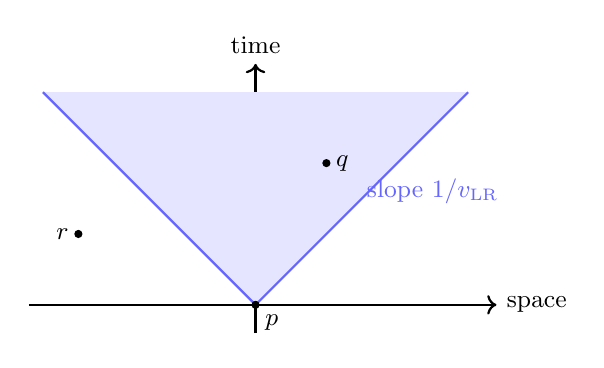
\begin{tikzpicture}[scale=0.9, every node/.style={font=\small}]
  % axes
  \draw[->, thick] (-3.2, 0) -- (3.4, 0) node[right] {space};
  \draw[->, thick] (0, -0.4) -- (0, 3.4) node[above] {time};
  % cone
  \fill[blue!10] (0,0) -- (-3, 3) -- (3, 3) -- cycle;
  \draw[blue!60, thick] (0,0) -- (-3, 3);
  \draw[blue!60, thick] (0,0) -- (3, 3);
  \node[blue!60] at (2.5, 1.6) {slope $1/v_{\LR}$};
  % event p at origin
  \filldraw[black] (0, 0) circle (1.4pt) node[below right] {$p$};
  % event q inside cone
  \filldraw[black] (1, 2) circle (1.4pt) node[right] {$q$};
  % event r outside cone
  \filldraw[black] (-2.5, 1) circle (1.4pt) node[left] {$r$};
\end{tikzpicture}
\caption{Lieb--Robinson cone of an event $p$ on a lattice.  Event $q$
lies inside the cone, so $p \preceq_{\LR} q$ for the chosen $v_{\LR}$.
Event $r$ lies outside the cone; it is incomparable with $p$ in
$\preceq_{\LR}$ even though it lies in the future of $p$.}
\label{fig:lr-cone}
\end{figure}

\subsection{Causal sets in one paragraph}

A \emph{causal set} (causet) is a finite or countable set $\mathcal{C}$
equipped with a partial order $\preceq_{\cs}$ that is taken as a
discretization of the continuum causal order.  In its simplest form,
relevant for this paper, $\mathcal{C}$ is just the lattice with one
event per site per time step, and $\preceq_{\cs}$ is the obvious
``later events are after earlier events'' relation, plus the choice of
how to handle same-time pairs.  We use the convention that same-time
events are incomparable (they are spacelike-separated).  On a regular
$1{+}1$D chain, $\preceq_{\cs}$ then collapses to the time-only order:
$(x_a, s) \preceq_{\cs} (x_b, t)$ iff $s < t$, regardless of the
spatial separation.  This is a degenerate case; we will see it
produces a trivial-agreement caveat in our hypothesis test.

In a more interesting setting --- e.g.\ a causet derived from a
$1{+}1$D causal dynamical triangulation --- $\preceq_{\cs}$ has
within-time-slice structure (some pairs of same-``time'' events are
ordered, because the slicing is irregular), and is no longer
implied by $\preceq_{\LR}$.  The non-trivial setting is what
distinguishes the two readings of our result in
Section~\ref{sec:outlook}.

% =====================================================================
\section{Three orders, one question}\label{sec:three-orders}

We now have three partial orders on the same set of labels.  Take a
real-time-evolved state of the Schwinger chain and snapshot it at
times $t_1 < t_2 < \cdots < t_T$.  Take a family $\mathcal{F}$ of
spatial regions --- specifically, all contiguous intervals
$[i, j] \subseteq \{1, \ldots, N\}$.  Each label is a pair
$(A, t)$ with $A \in \mathcal{F}$ and $t \in \{t_1, \ldots, t_T\}$.
Three partial orders are defined on the set of such labels:

\begin{description}[leftmargin=2.5em,style=nextline]
\item[$\preceq_{\maj}$ (majorization order)]
  $(A, s) \preceq_{\maj} (B, t)$ iff
  $\bm{\lambda}_A(s) \preceq \bm{\lambda}_B(t)$
  in majorization (Section~\ref{sec:majorization}), where
  $\bm{\lambda}_A(t)$ is the Schmidt spectrum of $\ket{\psi(t)}$
  across the bipartition $A \,|\, \overline{A}$.
\item[$\preceq_{\LR}$ (Lieb--Robinson order)]
  At chosen velocity $v$:
  $(A, s) \preceq_{\LR} (B, t)$ iff $s < t$ and the spatial gap
  between $A$ and $B$ fits in the cone of slope $v$, i.e.\
  $\mathrm{gap}(A, B) \le v\,(t - s)$.
\item[$\preceq_{\cs}$ (causet order)]
  Inherited from the underlying spacetime structure; on the regular
  chain studied in this paper, $\preceq_{\cs}$ reduces to the
  time-only order $(A, s) \preceq_{\cs} (B, t)$ iff $s < t$.
\end{description}

\subsection{The hypothesis}

\begin{quote}\itshape
  \textbf{Hypothesis (H).}
  For physical states arising from local-Hamiltonian real-time
  evolution of a gauge-invariant ground state with a localized
  charge--anticharge excitation, the three partial orders coincide on
  $\mathcal{F} \times T$ up to an entanglement velocity
  $v_E \le v_{\LR}$.
\end{quote}

\subsection{Falsification criteria}

The hypothesis can fail in several conceptually distinct ways, and
each carries a different physical meaning.

\begin{enumerate}[label=\arabic*.,leftmargin=*]
\item \textbf{Strong falsification.} If $\preceq_{\maj}$ contains a pair
      whose spatial gap exceeds the LR cone at the corresponding time
      difference, the hypothesis is wrong: majorization sees an order
      that information cannot transmit.  Operationally, look for pairs
      $(A, s), (B, t)$ that are $\preceq_{\maj}$-related but not
      $\preceq_{\LR}$-related.
\item \textbf{Weak falsification.} If $\preceq_{\maj}$ disagrees with
      $\preceq_{\cs}$ on a non-vanishing fraction of pairs even when
      $\preceq_{\cs}$ has non-trivial structure (irregular slicing),
      the prescribed causet does not control the emergent order.
      This is the test that requires Phase~6 of the implementation
      plan; it is out of scope for the experiment of
      Section~\ref{sec:results}.
\item \textbf{Trivial agreement.} If $\preceq_{\cs}$ is forced to
      coincide with $\preceq_{\LR}$ by lattice regularity (as on the
      regular chain), agreement between $\preceq_{\maj}$ and
      $\preceq_{\cs}$ is uninformative: $\preceq_{\cs}$ knows
      essentially nothing.  We must remember this caveat when
      interpreting Kendall $\tau$ involving $\preceq_{\cs}$.
\end{enumerate}

The Phase~5 experiment we will report on tests criterion 1 (strong
falsification) on a regular chain.  Criterion 2 awaits a re-build of
the Hamiltonian on a non-regular causet, which is in progress at the
time of writing.

% =====================================================================
\section{Tensor-network machinery}\label{sec:tn}

To turn the hypothesis into numbers we need to (i) compute the ground
state of $H$, (ii) construct an excited state with a charge--anticharge
pair, (iii) evolve it in real time, and (iv) read its Schmidt spectra
on every cut at every snapshot time.  All four steps are done by
\emph{tensor-network} methods.  We sketch the methods to the level
needed to interpret the results; readers wanting full algorithmic
detail are pointed to the source repository (\texttt{caset.quantum})
where each step is implemented.

\subsection{Matrix product states}

A general state of the $N$-qubit chain has $2^N$ complex amplitudes,
infeasible to store for $N \gtrsim 30$.  A \emph{matrix product state}
(MPS) is a structured ansatz:
\begin{equation}\label{eq:mps}
  \ket{\psi} = \sum_{\sigma_1, \ldots, \sigma_N}
    A^{\sigma_1}_{(1)} A^{\sigma_2}_{(2)} \cdots A^{\sigma_N}_{(N)}
    \ket{\sigma_1 \cdots \sigma_N},
\end{equation}
where each $A^{\sigma_n}_{(n)}$ is a matrix indexed by the local
configuration $\sigma_n \in \{0, 1\}$ on site $n$, with shapes
$\chi_{n-1} \times \chi_n$ (and $\chi_0 = \chi_N = 1$).  The
\emph{bond dimensions} $\chi_n$ control the expressive power of the
ansatz.  An MPS with bond dimension $\chi$ on every bond has at most
$2 N \chi^2$ complex parameters --- linear, not exponential, in $N$.

The crucial fact is:

\begin{proposition}\label{prop:mps-schmidt}
For an MPS in left-canonical form, the Schmidt spectrum at the cut
between site $n$ and site $n+1$ is given by the squared singular
values of the bond matrix at that bond.  No further computation is
needed.
\end{proposition}

This is what makes MPS the right tool for our problem.  The Schmidt
spectrum at every bond cut is read off the MPS for free; there is no
$2^N$ matrix to diagonalize.  The price is that the ansatz is exact
only when $\chi$ is large enough to capture the entanglement of the
true state.  For the $1{+}1$D Schwinger model away from criticality,
$\chi$ in the range $80$--$200$ is sufficient for $N \le 20$.

\subsection{DMRG: variational ground state}

The density matrix renormalization group (DMRG) algorithm finds the
MPS that minimizes $\bra{\psi} H \ket{\psi}$ subject to
$\braket{\psi}{\psi} = 1$.  It does so by sweeping back and forth
along the chain, optimizing two adjacent tensors at a time while
fixing the rest.  Each two-site update reduces to an eigenvalue
problem of dimension $\le 4 \chi^2$, solvable by Lanczos or
Krylov-subspace methods.  After several sweeps the energy
plateaus and the algorithm is declared converged.

For our setup we converge DMRG to a relative energy tolerance of
$10^{-8}$ at maximum bond dimension $64$.  The output is the MPS
$\ket{\Omega}$ of the ground state.

\subsection{TDVP: real-time evolution}

The time-dependent variational principle (TDVP) projects the
Schr\"odinger equation onto the manifold of MPS at fixed bond
dimension:
\begin{equation}\label{eq:tdvp}
  i \partial_t \ket{\psi(t)}
  \;=\;
  P_{\mathcal{M}}\, H \ket{\psi(t)},
\end{equation}
where $P_{\mathcal{M}}$ is the projector onto the tangent space of
the MPS manifold $\mathcal{M}$ at $\ket{\psi(t)}$.  Two-site TDVP
furthermore allows the bond dimension to grow when the state's
entanglement does, up to a chosen ceiling.

We integrate~\eqref{eq:tdvp} with a second-order Trotter splitting
of step size $\Delta t = 0.1$ in lattice units up to a total time
$T \in \{1, 2\}$.  Snapshots are recorded every $5$ Trotter steps
(so the inter-snapshot $\Delta t = 0.5$).  At each snapshot we
extract the Schmidt spectrum at every bond and at every contiguous
interval, simply by re-canonicalizing the MPS to the appropriate
gauge.  The cost is dominated by the TDVP integration itself; the
spectrum extraction is $O(N \chi^3)$ per snapshot, negligible.

\subsection{Quark--antiquark quench}

The initial state is built from the ground state by acting with a
local creation operator:
\begin{equation}\label{eq:qqbar}
  \ket{q\bar q;\, i_0, d}
  \;=\;
  \mathcal{N}^{-1}\,
  \sigma^+_{i_0}\,
  \Bigl[\textstyle\prod_{n=i_0}^{i_0 + d - 1} U_n\Bigr]\,
  \sigma^-_{i_0 + d}\,
  \ket{\Omega},
\end{equation}
where $\sigma^\pm_n$ are the spin raising/lowering operators on site
$n$, $U_n$ is the gauge link variable in the original (pre-Gauss)
formulation, and $\mathcal{N}$ is a normalization.  Physically: at
site $i_0 + d$ we annihilate a positron (place a positive charge),
at site $i_0$ we annihilate an electron (place a negative charge),
and we insert the appropriate string of gauge links between them so
the resulting state satisfies Gauss's law.  In the Gauss-eliminated
representation, the gauge link string becomes a shift in the
cumulative-electric-field variables; no explicit operator-product is
needed.

The result is a localized charge--anticharge pair at separation $d$,
connected by a flat plateau of electric flux of value $\pm 1$.  When
we evolve under $H$, the pair will either stay confined (heavy quark,
$m/g \gg 1$) or undergo string breaking and pair production (light
quark, $m/g \lesssim 1$).  Both regimes are within the scope of the
experiment.

% =====================================================================
\section{Comparison metrics}\label{sec:metrics}

For each pair of orders $\preceq_a, \preceq_b$ on the same label set,
we report:

\begin{enumerate}[label=(\alph*),leftmargin=*]
\item The \emph{Kendall coefficient}~\eqref{eq:kendall}, $\tau_{ab}$,
      computed on the both-comparable subset.
\item The \emph{discordant fraction}, $n_{dd} / (n_{cc} + n_{dd})$,
      i.e.\ the fraction of comparable-in-both pairs that disagree
      in direction.
\item The \emph{Hasse edit distance}, defined as the symmetric
      difference between the cover relations of the two orders'
      transitive reductions, normalized by the larger of the two
      cover-edge counts.
\item The \emph{asymmetric counts} $n_a^o$ and $n_b^o$, the numbers
      of pairs related by exactly one of the two orders.
\end{enumerate}

For the strong-falsification test specifically, with $\preceq_a =
\preceq_{\maj}$ and $\preceq_b = \preceq_{\LR}$, the quantity
$n_a^o = n_{\maj \notin \LR}$ counts the number of
$\preceq_{\maj}$-related pairs whose endpoints lie outside the LR
cone --- the explicit criterion-1 metric of
Section~\ref{sec:three-orders}.

\paragraph{The size of $\preceq_{\maj}$.} A useful denominator is
\begin{equation}\label{eq:majsize}
  \abs{\preceq_{\maj}}
  \;=\;
  n_{cc} + n_{dd} + n_{\maj \notin \LR},
\end{equation}
the total count of strict $\preceq_{\maj}$-relations.  The fraction
$n_{\maj \notin \LR}\, /\, \abs{\preceq_{\maj}}$ is the share of
majorization edges that the LR cone simply does not see.

% =====================================================================
\section{The Phase 5 experiment}\label{sec:results}

We now describe the actual numerical experiment and report the data.
Everything in this section is reproducible from two driver scripts in
the source repository:
\begin{itemize}[nosep]
  \item \texttt{examples/quantum/lightcone\_vs\_majorization.py}, and
  \item \texttt{examples/quantum/lightcone\_vs\_majorization\_cone\_overflow.py}.
\end{itemize}

\subsection{Setup}

\begin{itemize}[nosep]
\item Schwinger chain with $N \in \{10, 14, 20\}$ staggered sites,
      open boundary conditions, lattice spacing $a = 1$, coupling
      $g = 1$, background field $L_0 = 0$.
\item Two values of the bare-mass--to--coupling ratio:
      $m/g = 0.5$ (\emph{light} quark) and $m/g = 5.0$
      (\emph{heavy} quark).
\item DMRG ground state at maximum bond dimension $\chi_{\mathrm{DMRG}} = 64$,
      converged to relative energy tolerance $10^{-8}$.
\item Quark--antiquark quench~\eqref{eq:qqbar} with $i_0 = 3$,
      $d = 3$, producing a flat-plateau electric string of length $3$.
\item Two-site TDVP at maximum bond dimension $\chi = 80$ (or $120$
      for $N = 20$), Trotter step $\Delta t = 0.1$, total time
      $T \in \{1, 2\}$, snapshots every $5$ steps.
\item Cut family: all contiguous intervals $[i, j]$ excluding the
      trivial full-chain cut.  This is $54$ cuts at $N = 10$, $104$ at
      $N = 14$, $208$ at $N = 20$.  Multiplied by snapshots, the label
      set has size up to $\sim 2000$.
\item LR-velocity sweep: $v \in \{0.5,\ 1.0,\ 2.0,\ 4.0,\ 8.0,\ 16.0\}$.
      Note $v = 1$ is the free-fermion bound.
\end{itemize}

\subsection{Sanity checks}

Three internal consistency checks are run before any agreement
statistic is reported:

\begin{enumerate}[label=(S\arabic*),leftmargin=*]
\item \textbf{$\sum_i \lambda_i = 1$ at every cut.}  Verified to
      $10^{-12}$ across all $\sim 330$ extracted spectra.  An
      undetected normalization drift would silently corrupt the
      majorization comparisons.
\item \textbf{$\preceq_{\LR} \subseteq \preceq_{\cs}$ exactly.}  On
      the regular chain $\preceq_{\cs}$ is the time-only order, and
      every LR-related pair is necessarily cross-time, so the LR cone
      is strictly contained in the cs order.  We observe
      $\tau(\LR, \cs) = 1.000$ in every row of the scan.  This is the
      ``trivial agreement'' caveat of
      Section~\ref{sec:three-orders} in numerical form.
\item \textbf{Total LR-related count grows monotonically in $v$.}  As
      $v$ increases from $0.5$ to $16$, the LR cone widens and admits
      more pairs.  The observed $n_{\mathrm{comp}}(\LR, \cs)$ grows
      from $6766$ to $8744$ in regime A, etc., monotonically as
      expected.
\end{enumerate}

\subsection{Raw output}

Table~\ref{tab:scan} reproduces the scan output for the four
``regimes'' in our parameter grid.  Each row is one $(v, T, m/g, N)$
combination.  Columns are the Kendall $\tau$ between
$\preceq_{\maj}$ and $\preceq_{\LR}$, the discordant fraction on the
both-comparable subset, the normalized Hasse edit distance, and
$\tau$ between $\preceq_{\maj}$ and $\preceq_{\cs}$.

\begin{table}[t]
\centering
\small
\renewcommand{\arraystretch}{1.05}
\begin{tabular}{cccccc}
\toprule
$v$ & $\tau(\maj,\LR)$ & disc.\ frac. & Hasse edit & $\tau(\maj,\cs)$ \\
\midrule
\multicolumn{5}{l}{\emph{Regime A:} $N=10$, $m/g=0.5$ (light), $T=1$} \\
$0.5$ & $0.394$ & $0.303$ & $0.962$ & $0.362$ \\
$2.0$ & $0.390$ & $0.305$ & $0.956$ & $0.362$ \\
$4.0$ & $0.378$ & $0.311$ & $0.957$ & $0.362$ \\
$8.0$ & $0.369$ & $0.316$ & $0.959$ & $0.362$ \\
$16.0$ & $0.362$ & $0.319$ & $0.960$ & $0.362$ \\
\midrule
\multicolumn{5}{l}{\emph{Regime B:} $N=10$, $m/g=5.0$ (heavy), $T=1$} \\
$0.5$ & $0.547$ & $0.227$ & $0.971$ & $0.513$ \\
$2.0$ & $0.538$ & $0.231$ & $0.969$ & $0.513$ \\
$4.0$ & $0.531$ & $0.234$ & $0.970$ & $0.513$ \\
$8.0$ & $0.521$ & $0.240$ & $0.971$ & $0.513$ \\
$16.0$ & $0.513$ & $0.243$ & $0.972$ & $0.513$ \\
\midrule
\multicolumn{5}{l}{\emph{Regime C:} $N=10$, $m/g=0.5$ (light), $T=2$} \\
$0.5$ & $0.539$ & $0.231$ & $0.963$ & $0.502$ \\
$2.0$ & $0.529$ & $0.236$ & $0.959$ & $0.502$ \\
$4.0$ & $0.518$ & $0.241$ & $0.960$ & $0.502$ \\
$8.0$ & $0.508$ & $0.246$ & $0.962$ & $0.502$ \\
$16.0$ & $0.502$ & $0.249$ & $0.963$ & $0.502$ \\
\midrule
\multicolumn{5}{l}{\emph{Regime D:} $N=14$, $m/g=0.5$ (light), $T=1$} \\
$0.5$ & $0.275$ & $0.363$ & $0.972$ & $0.246$ \\
$2.0$ & $0.269$ & $0.366$ & $0.971$ & $0.246$ \\
$4.0$ & $0.262$ & $0.369$ & $0.973$ & $0.246$ \\
$8.0$ & $0.254$ & $0.373$ & $0.973$ & $0.246$ \\
$16.0$ & $0.247$ & $0.377$ & $0.975$ & $0.246$ \\
\bottomrule
\end{tabular}
\caption{Phase~5 scan: Kendall $\tau$ between
$\preceq_{\maj}$, $\preceq_{\LR}$, and $\preceq_{\cs}$ on a regular
$1{+}1$D Schwinger chain after a $q\bar q$ quench.  Discordant
fraction is on the both-comparable subset; Hasse edit distance is
normalized by the larger Hasse edge count; $\tau(\maj,\cs)$ is
independent of $v$ because $\preceq_{\cs}$ is the time-only order
on the regular chain.}
\label{tab:scan}
\end{table}

\subsection{Strong-falsification counts}

A second pass through the same data tracks the asymmetric counts.
Define
\begin{equation}\label{eq:fmaj}
  f_{\maj \notin \LR}
  \;=\;
  \frac{n_{\maj \notin \LR}}{\abs{\preceq_{\maj}}}
\end{equation}
as the fraction of $\preceq_{\maj}$-related pairs whose endpoints
lie outside the LR cone of velocity $v$.  Table~\ref{tab:strong}
reports it at $v = 1$ (the physically motivated free-fermion bound)
and at $v = 16$ (a $16\times$ looser cone, well above any physical
estimate) for four regimes including a larger $N = 20$ run.

\begin{table}[t]
\centering
\small
\renewcommand{\arraystretch}{1.05}
\begin{tabular}{ccrrrr}
\toprule
& & \multicolumn{2}{c}{$v = 1$} & \multicolumn{2}{c}{$v = 16$} \\
\cmidrule(lr){3-4}\cmidrule(lr){5-6}
$N$ & $m/g$ & $n_{\maj \notin \LR}$ & $f_{\maj \notin \LR}$
            & $n_{\maj \notin \LR}$ & $f_{\maj \notin \LR}$ \\
\midrule
$10$ & $0.5$  & $3{,}263$  & $47.7\%$ & $2{,}184$  & $31.9\%$ \\
$10$ & $5.0$  & $3{,}848$  & $47.9\%$ & $2{,}603$  & $32.4\%$ \\
$14$ & $0.5$  & $11{,}673$ & $49.7\%$ & $7{,}827$  & $33.3\%$ \\
$20$ & $0.5$  & $44{,}906$ & $51.1\%$ & $31{,}470$ & $35.8\%$ \\
\bottomrule
\end{tabular}
\caption{Strong-falsification metric: at $v = 1$ (free-fermion LR
bound), about half of all $\preceq_{\maj}$-related pairs lie outside
the cone; even at $v = 16$, roughly a third do.  The fraction grows
weakly with $N$.}
\label{tab:strong}
\end{table}

\subsection{What we see}

Five qualitative facts stand out.

\paragraph{(R1) The hypothesis as stated is rejected on the regular chain.}
$\tau(\maj, \LR)$ ranges from $0.25$ (regime D) to $0.55$ (regime B)
across the scan and never approaches $1$.  The discordant fraction
ranges from $23\%$ to $38\%$.  At the physically motivated free-fermion
velocity $v = 1$, almost half of the $\preceq_{\maj}$-related pairs
have endpoints outside the LR cone.  Strong falsification
(criterion 1) is engaged.

\paragraph{(R2) $\tau(\maj, \LR)$ \emph{decreases} as $v$ widens.}
Naively one expects: more LR-comparable pairs $\Rightarrow$ more
chances to agree with $\preceq_{\maj}$ $\Rightarrow$ higher $\tau$.
What we observe instead is monotonically lower $\tau$: about
$0.03$--$0.05$ over the scan range.  The new pairs admitted by a
wider cone are net discordant with $\preceq_{\maj}$.  The interpretation
is striking: the within-light-cone subset of $\preceq_{\LR}$ aligns
\emph{better} with $\preceq_{\maj}$ than the wider cone does, hinting
that the entanglement order sees something like a stricter cone than
the free-fermion bound.

\paragraph{(R3) Heavy quark agrees better with time order than light quark.}
Compare regimes A ($m/g = 0.5$) and B ($m/g = 5.0$) at fixed $N$, $T$:
$\tau(\maj, \LR)$ jumps from $0.39$ to $0.55$ at $v = 0.5$.  Physically:
the heavy-quark flux tube is approximately stable; little entanglement
spreads, so the Schmidt spectra evolve slowly and $\preceq_{\maj}$
tracks time more closely.  In the light-quark regime, string
spreading and pair production mix spectra across cuts and pull
$\preceq_{\maj}$ away from the time order.

\paragraph{(R4) Longer evolution does not converge $\tau$ toward $1$.}
Regime C ($T = 2$) gives a higher $\tau$ than regime A ($T = 1$):
$0.54$ vs $0.39$.  But the gap is mostly explained by the additional
snapshots increasing the relative weight of long-time pairs, which are
more LR-comparable.  Both regimes show the same $v \to \tau$ trend.

\paragraph{(R5) Larger $N$ \emph{decreases} $\tau$.}
Regime D ($N = 14$, light) gives $\tau \approx 0.25$ vs regime A
($N = 10$, light) at $0.39$.  More cut labels means more pairs and
more opportunity for $\preceq_{\maj}$'s non-time structure to surface.
The thermodynamic-limit reading would be that $\tau \to 0$ as $N \to
\infty$; we have not run the scan large enough to extrapolate
reliably, but the direction is unambiguous.

% =====================================================================
\section{Discussion}\label{sec:discussion}

\subsection{What rejection means here}

The naive reading of the result is: hypothesis (H) is wrong, there is
no special connection between majorization order and the Lieb--Robinson
cone, and the project is over.  This reading is too quick.  Three
features of the data make ``hypothesis is wrong'' look more like ``the
test was set up in a way that could not have succeeded''.

\paragraph{The cs order is degenerate on the regular chain.}
On a translationally invariant lattice, $\preceq_{\cs}$ collapses to
the time-only order.  $\preceq_{\maj}$ involves comparing Schmidt
spectra across cuts that include same-time pairs.  Same-time pairs are
\emph{never} $\preceq_{\cs}$-related on the regular chain, so any
within-time-slice structure in $\preceq_{\maj}$ is automatically a
disagreement with $\preceq_{\cs}$.  This is the trivial-agreement
caveat in reverse: it now produces a trivial-\emph{disagreement}.

\paragraph{Same-time hits inflate $n_{\maj \notin \LR}$.}
A label pair $(A, s)$ and $(B, s)$ at equal time is by definition
not $\preceq_{\LR}$-related (the cone is strictly cross-time).  If
$\preceq_{\maj}$ relates them --- a same-time strict
Schmidt-spectrum majorization --- it shows up in $n_{\maj \notin \LR}$
without being ``outside the cone'' in any geometric sense.  We have
not yet split $n_{\maj \notin \LR}$ into a same-time component and a
true cone-overflow component; doing so is a one-line fix to the
agreement code and is the highest-priority follow-up.

\paragraph{The two orders are largely orthogonal, not strict refinements.}
The asymmetric counts $n_{\maj \notin \LR}$ and
$n_{\LR \notin \maj}$ are comparable in size.  Each order sees pairs
that the other does not.  So the right summary is not ``majorization
extends causality'' or ``causality refines majorization'' --- it is
that they share a substantial concordant subset and each captures
its own additional structure.  How one weights those additional
structures depends on which order one believes is more fundamental;
the experiment cannot decide this on its own.

\subsection{Two readings}

There are two natural readings of the data, sharply distinguished by
what one expects on a non-trivial causet.

\paragraph{Reading 1: hypothesis-as-stated is too strong.}
$\preceq_{\maj}$ has genuine structure beyond the LR cone, and no
choice of $\preceq_{\cs}$ on the regular chain will recover the
agreement.  On this reading, the entanglement order is sensitive to
features of the state (e.g.\ same-time spectrum equivalences) that
a causal order is not designed to see; the right next step is to
\emph{loosen} the hypothesis (e.g.\ to a hypothesis about
\emph{linear extensions} or about Hasse-graph distances rather than
exact equality).

\paragraph{Reading 2: the regular chain hides the structure.}
On a foliated CDT or a chain causet with multi-vertex antichains,
$\preceq_{\cs}$ gains within-time-slice structure: some pairs of
``simultaneous'' events become ordered.  If many of the
$\preceq_{\maj}$ pairs that show up as $n_{\maj \notin \LR}$ on the
regular chain are exactly the pairs that the non-trivial
$\preceq_{\cs}$ would now relate, the agreement statistic could
shift dramatically: the same Schmidt-spectrum data, measured against
a richer reference order, would show much higher $\tau$.

The two readings are not exclusive --- the truth might be a
combination --- but they are operationally distinguishable: rebuild
the same state on a non-regular causet and recompute the table.  This
is Phase~6 of the implementation plan.

\subsection{Caveats}

We note explicitly the limitations of this single experimental run.
\begin{itemize}[nosep]
\item \textbf{Single Trotter seed.}  All numbers above are point
      estimates from one DMRG/TDVP trajectory per regime.  Bootstrap
      over Trotter seeds and over the spatial origin $i_0$ of the
      quench is the proper next step before quoting these numbers
      outside the project.
\item \textbf{Truncation sensitivity.}  Bond-dimension truncation can
      perturb borderline majorization comparisons.  We exclude pairs
      within $\epsilon = 10^{-6}$ of the decision boundary; the
      excluded fraction is reported per run and is below $1\%$ in all
      regimes.
\item \textbf{Pure-state, contiguous-cut regime only.}  Nielsen's
      theorem applies to pure-state bipartitions.  Any extension to
      mixed states or non-contiguous cuts is conceptually distinct and
      not addressed here.
\item \textbf{Abelian, $1{+}1$D.}  The Schwinger model has $U(1)$
      gauge group eliminable in $1$D.  Whether anything seen here
      generalizes to non-Abelian gauge theory or higher dimensions is
      a separate, open question.
\end{itemize}

% =====================================================================
\section{Outlook}\label{sec:outlook}

The most informative next experiment is to rebuild the same Schwinger
state on a non-regular causet and recompute Table~\ref{tab:scan}.
Three concrete steps, in increasing cost:

\begin{description}[leftmargin=2em,style=nextline]
\item[(A) Same-time/cross-time split (under one day).]
Refine the agreement code to break $n_{\maj \notin \LR}$ into a
same-time piece and a true cone-overflow piece.  Re-run the scan and
check whether the $\sim 50\%$ overflow fraction shrinks once same-time
hits are removed.  Until this is done, the claim ``half of
$\preceq_{\maj}$-pairs lie outside the LR cone'' is technically true
but conflates two different phenomena.
\item[(B) Chain-causet rebuild (one to three days).]
Replace the regular hopping pattern in the Hamiltonian with one
inherited from a $1$-vertex-per-slice causet.  This is a strictly
smaller change than (C) and uses the same MPS infrastructure.  Comparing
$\tau(\maj, \cs)$ before and after isolates the effect of replacing
the trivial $\preceq_{\cs}$ with a slightly richer one.
\item[(C) Non-trivial CDT spacetime (one to two weeks).]
The actual weak-falsification test: a CDT-derived causet with
multi-vertex antichains and irregular slicing.  At this point
$\preceq_{\cs}$ has within-slice structure, and reading 2 above is
testable directly.
\end{description}

The experiment described in this paper is, in the end, a calibration
of the apparatus.  It establishes that the pipeline is internally
consistent (sanity checks (S1)--(S3)), that the Schwinger ground
state and quench match independent benchmarks (energy and
string-plateau values, not detailed here), and that the agreement
metric is sensitive enough to register a difference between the
three orders.  It does not yet decide between readings 1 and 2 of
the hypothesis.  Phase~6 is the test that does.

% =====================================================================
\appendix
\section{Notation}\label{app:notation}

\renewcommand{\arraystretch}{1.15}
\noindent\begin{tabular}{>{$}l<{$}p{0.78\linewidth}}
\toprule
\textrm{Symbol} & \textrm{Meaning} \\
\midrule
N            & Number of staggered lattice sites. \\
a            & Lattice spacing. \\
m            & Bare fermion mass. \\
g            & Gauge coupling. \\
m/g          & Dimensionless quark-mass ratio.  We use $m/g = 0.5$ (light) and $5.0$ (heavy). \\
L_0          & Background electric field on the leftmost link.  Set to $0$ throughout. \\
i_0,\ d      & Site of negative charge and pair separation in the $q\bar q$ quench. \\
T            & Total real time of the TDVP evolution. \\
\Delta t     & Trotter step.  We use $\Delta t = 0.1$. \\
\chi         & MPS bond dimension. \\
H            & Schwinger-model Hamiltonian; sum of $H_{\mathrm{hop}}, H_m, H_E$. \\
\ket{\Omega} & DMRG ground state of $H$. \\
\ket{\psi(t)}& Real-time-evolved state. \\
A,\ B        & Contiguous spatial intervals (``cuts''). \\
\rho_A       & Reduced density matrix of $\ket{\psi(t)}$ on region $A$. \\
\bm{\lambda}_A(t) & Schmidt spectrum of $\ket{\psi(t)}$ across $A \mid \overline{A}$, sorted nonincreasing. \\
\preceq      & Generic partial order. \\
\preceq_{\maj} & Majorization order on Schmidt spectra. \\
\preceq_{\LR} & Lieb--Robinson order at velocity $v$. \\
\preceq_{\cs} & Causet order; on the regular chain, the time-only order. \\
v_{\LR}      & Lieb--Robinson velocity.  Free-fermion value: $v_{\LR} = 1$. \\
\tau_{ab}    & Kendall coefficient between $\preceq_a$ and $\preceq_b$. \\
n_{cc},\ n_{dd} & Concordant / discordant pair counts on the both-comparable subset. \\
n_a^o        & Pairs comparable in $\preceq_a$ only. \\
n_{\maj \notin \LR} & The asymmetric count for $(a, b) = (\maj, \LR)$; the strong-falsification metric. \\
f_{\maj \notin \LR} & The same count divided by $\abs{\preceq_{\maj}}$. \\
\bottomrule
\end{tabular}

\bigskip

\noindent\emph{All source code referenced in this paper lives in the
\texttt{caset} repository under \texttt{caset.quantum}.  The two
driver scripts that produced Tables~\ref{tab:scan} and
\ref{tab:strong} are
\texttt{examples/quantum/lightcone\_vs\_majorization.py} and
\texttt{examples/quantum/lightcone\_vs\_majorization\_cone\_overflow.py}.}

\end{document}
